%%%%%%%%%%%%%%%%%%%%%%%%%%%%% Define Article %%%%%%%%%%%%%%%%%%%%%%%%%%%%%%%%%%
\documentclass{article}
%%%%%%%%%%%%%%%%%%%%%%%%%%%%%%%%%%%%%%%%%%%%%%%%%%%%%%%%%%%%%%%%%%%%%%%%%%%%%%%

%%%%%%%%%%%%%%%%%%%%%%%%%%%%% Using Packages %%%%%%%%%%%%%%%%%%%%%%%%%%%%%%%%%%
\usepackage[utf8]{inputenc}
\usepackage{float, geometry, graphicx, fancyhdr, color, xcolor}
\usepackage{amssymb, amsthm, amsmath, tikz, pgfplots, comment, wrapfig}
\usepackage{listings, mdframed, lipsum, psfrag, parskip, empheq, subfig, verbatim}
\usepackage[english]{babel}
\usepackage[breaklinks]{hyperref}
\usepackage{titlesec, cite, hyperref, wrapfig, booktabs, bookmark, pdfpages}

%%%%%%%%%%%%%%%%%%%%%%%%%%%%%%%%%%%%%%%%%%%%%%%%%%%%%%%%%%%%%%%%%%%%%%%%%%%%%%%

%%%%%%%%%%%%%%%%%%%%%%%%%% C Code Listing Settings %%%%%%%%%%%%%%%%%%%%%%%%%%%%%%%%%%%%%%%
\definecolor{mGreen}{rgb}{0.25,0.63,0.15}
\definecolor{mGray}{rgb}{0.5,0.5,0.5}
\definecolor{mPurple}{rgb}{0.58,0,0.82}
\definecolor{codeBlue}{rgb}{0.01, 0.2, 0.92}
\definecolor{codegray}{rgb}{0.5,0.5,0.5}
\definecolor{codepurple}{rgb}{0.58,0,0.82}
\definecolor{codeblue}{rgb}{0.13,0.29,0.53}
\definecolor{backgroundColour}{rgb}{0.95,0.95,0.95}

\lstset{
    language=Python,
    backgroundcolor=\color{backgroundColour},
    basicstyle=\ttfamily\small,
    commentstyle=\color{deepGreen},
    keywordstyle=\color{blue},
    numberstyle=\tiny\color{mGray},
    stringstyle=\color{red},
    breakatwhitespace=false,         
    breaklines=true,                 
    captionpos=b,                    
    keepspaces=true,                 
    numbers=left,                    
    numbersep=5pt,                  
    showspaces=false,                
    showstringspaces=false,
    showtabs=false,                  
    tabsize=2,
    frame=single
}

%%%%%%%%%%%%%%%%%%%%%%%%%%%%%%%%%%%%%%%%%%%%%%%%%%%%%%%%%%%%%%%%%%%%%%%%%%%%%%%

% Other Settings
\hypersetup{
    colorlinks = true,
    linkcolor = black,
    urlcolor = blue,
}
\urlstyle{same}

%%%%%%%%%%%%%%%%%%%%%%%%%% Page Setting %%%%%%%%%%%%%%%%%%%%%%%%%%%%%%%%%%%%%%%
\geometry{a4paper}
\pagestyle{fancy}
\fancyhead{}
\fancyhead[L]{Computational Intelligence}
\fancyhead[C]{Assignment 02 - Report}
\fancyhead[R]{CS 451}
\fancyfoot{}
\fancyfoot[C]{\thepage \;of }

%%%%%%%%%%%%%%%%%%%%%%%%%% Define some useful colors %%%%%%%%%%%%%%%%%%%%%%%%%%
\definecolor{ocre}{RGB}{243,102,25}
\definecolor{mygray}{RGB}{243,243,244}
\definecolor{deepGreen}{RGB}{26,111,0}
\definecolor{shallowGreen}{RGB}{235,255,255}
\definecolor{deepBlue}{RGB}{61,124,222}
\definecolor{shallowBlue}{RGB}{235,249,255}
%%%%%%%%%%%%%%%%%%%%%%%%%%%%%%%%%%%%%%%%%%%%%%%%%%%%%%%%%%%%%%%%%%%%%%%%%%%%%%%

%%%%%%%%%%%%%%%%%%%%%%%%%% Define an orangebox command %%%%%%%%%%%%%%%%%%%%%%%%
\newcommand\orangebox[1]{\fcolorbox{ocre}{mygray}{\hspace{1em}#1\hspace{1em}}}
%%%%%%%%%%%%%%%%%%%%%%%%%%%%%%%%%%%%%%%%%%%%%%%%%%%%%%%%%%%%%%%%%%%%%%%%%%%%%%%

%%%%%%%%%%%%%%%%%%%%%%%%%%%% English Environments %%%%%%%%%%%%%%%%%%%%%%%%%%%%%
\newtheoremstyle{mytheoremstyle}{3pt}{3pt}{\normalfont}{0cm}{\rmfamily\bfseries}{}{1em}{{\color{black}\thmname{#1}~\thmnumber{#2}}\thmnote{\,--\,#3}}
\newtheoremstyle{myproblemstyle}{3pt}{3pt}{\normalfont}{0cm}{\rmfamily\bfseries}{}{1em}{{\color{black}\thmname{#1}~\thmnumber{#2}}\thmnote{\,--\,#3}}
\theoremstyle{mytheoremstyle}
\newmdtheoremenv[linewidth=1pt,backgroundcolor=shallowGreen,linecolor=deepGreen,leftmargin=0pt,innerleftmargin=20pt,innerrightmargin=20pt,]{theorem}{Theorem}[section]
\theoremstyle{mytheoremstyle}
\newmdtheoremenv[linewidth=1pt,backgroundcolor=shallowBlue,linecolor=deepBlue,leftmargin=0pt,innerleftmargin=20pt,innerrightmargin=20pt,]{definition}{Definition}[section]
\theoremstyle{myproblemstyle}
\newmdtheoremenv[linecolor=black,leftmargin=0pt,innerleftmargin=10pt,innerrightmargin=10pt,]{problem}{Problem}[section]
%%%%%%%%%%%%%%%%%%%%%%%%%%%%%%%%%%%%%%%%%%%%%%%%%%%%%%%%%%%%%%%%%%%%%%%%%%%%%%%

\title{{\huge \textbf{Habib University \\ Computational Intelligence - CS 451}}

\vspace*{5mm}
{\LARGE \textbf{Assignment 02 - Report} \\ \textbf{Swarm Intelligence}}
{
\includegraphics[width=0.75\linewidth]{logo.png}} \\ 
{\Large \textbf{Instructor:} Dr. Saleha Raza}}
\author{Ali Muhammad Asad - aa07190 \\ Dua Batool - db07098}
\date{}

\pgfplotsset{compat=1.18}

\begin{document}
\maketitle

\newpage
\tableofcontents

\newpage
\section{Question 1 - Graph Coloring Problem using Ant Colony Optimization}
\subsection{Introduction and Problem Formulation}
The Graph Coloring Problem is a well known problem in Computer Science that asks a really simple question, "What is the minimum number of colors required to color a graph such that no two adjacent vertices have the same color?". This problem is NP-Hard, a combinatorial optimization problem, and has a lot of real world applications. The image below shows a graph and its corresponding coloring.
\begin{figure}[htbp]
    \centering
    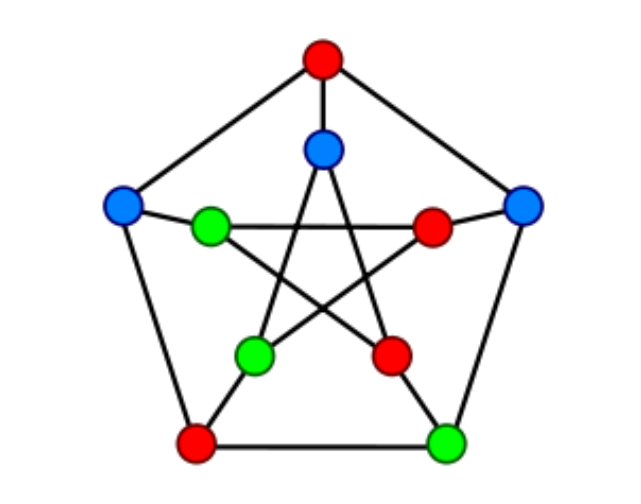
\includegraphics[width=0.35\textwidth]{../gco.png}
    \caption{Graph Coloring Example}
\end{figure}

In this assignment, the Ant Colony Optimization (ACO) Algorithm is used to efficiently provide a solution for coloring of a graph with minimum number of colors. The ACO algorithm is a probabilistic technique for solving computational problems which can be reduced to finding good paths through graphs. The ACO algorithm is inspired by the foraging behavior of ants and is a class of optimization algorithms that are based on the behavior of ants.

The problem can be formally formulated as follows:
\begin{definition}
    Given a graph $G = (V, E)$, where $V$ is the set of vertices and $E$ is the set of edges, a $k$-coloring of $G$ is a mapping such that $c: V \to \{ 1, 2, 3, ..., k \} $ is a mapping from the set of vertices to the set of colors such that $ \forall u, v \in V, \{ u, v \} \in E $ where $ \{u, v\} $ represents an edge from vertex $u$ to vertex $v$, $c(u) \neq c(v)$. The objective is to find the minimum value of $k$ such that a $k$-coloring of $G$ exists.
\end{definition}

We invoke the help of a theorem in Graph Theory for our implementation which makes things much easier for us, and helps us get to the solution faster. The theorem is as follows:
\begin{theorem}
    If $G$ is a simple graph with the largest vertex degree $ \triangle $, then $G$ is $ (\triangle + 1) $-colorable.
\end{theorem}
The above theorem is used in the color assignments, due to which the color assignement is initially sub-optimal, and not equal to the number of nodes, thus we get to an optimal solution much faster.

\subsection{Implementation of the Ant Colony Optimization Algorithm}
\subsubsection{Parameters}
\subsubsection{Graph Class}
\subsubsection{Ant Class}
\subsubsection{Ant Colony Class}

\subsection{Results and Analysis}

\end{document}
